\documentclass{article}
\usepackage[utf8]{inputenc}
\usepackage{float}
\usepackage[spanish]{babel}
\usepackage{graphicx}
\usepackage{listings}
\usepackage{color}
\usepackage{datetime}
\usepackage{csquotes}
\newdate{date}{19}{03}{2019}

\title{Tarea 3}
\author{Jesus Angel Patlán Castillo (5261)}
\date{\displaydate{date}}



\begin{document}

\definecolor{codegreen}{rgb}{0,0.6,0}
\definecolor{codegray}{rgb}{0.5,0.5,0.5}
\definecolor{codepurple}{rgb}{0.58,0,0.82}
\definecolor{backcolour}{rgb}{0.95,0.95,0.92}
 
\lstdefinestyle{mystyle}{
    backgroundcolor=\color{backcolour},   
    commentstyle=\color{codegreen},
    keywordstyle=\color{magenta},
    numberstyle=\tiny\color{codegray},
    stringstyle=\color{codepurple},
    basicstyle=\footnotesize,
    breakatwhitespace=false,         
    breaklines=true,                 
    captionpos=b,                    
    keepspaces=true,                 
    numbers=left,                    
    numbersep=5pt,                  
    showspaces=false,                
    showstringspaces=false,
    showtabs=false,                  
    tabsize=2
}
 
\lstset{style=mystyle}


\maketitle

En esta tarea se analizan 5 distintos algoritmos en grafos midiendo su tiempo de ejecución en base a grafos realizados tareas anteriores. Los algoritmos se obtuvieron por medio de la librería NetworkX \cite{NetworkX} de Python \cite{Python}, la librería Matplotlib \cite{Matplotlib} es utilizada para generar las gráficas de comparación entre los distintos algoritmos estudiados. El código empleado se obtuvo consultando la documentación oficial de la librería NetworkX \cite{NetworkXD}. Las imágenes y el código se encuentran disponibles directamente en mi repositorio \cite{JAPC}.

\section{Metodología}
La librería NetworkX tiene a la mano diversos algoritmos para resolver distintos problemas que se pueden presentar en los grafos. Particularmente para esta investigación, se realiza el análisis de los algoritmos:
\begin{itemize}
\item{Ruta más corta}: El algoritmo de la ruta más corta, como lo dice el nombre del algoritmo, trata de buscar la ruta más corta entre dos nodos dentro de un grafo. En la librería de NetworkX esta disponible por medio de  la función ``all shortest paths(G,N1,N2)", donde el parámetro G es el grafo, N1 el nodo origen y N2 el nodo destino:
\lstinputlisting[language=Python,firstline=102,lastline=102]{T3.py}
\item{Árbol búsqueda a profundidad}:  El algoritmo de árbol búsqueda a profundidad recorre el grafo dado para generar un árbol por medio de una búsqueda a profundidad. En la librería de NetworkX esta disponible por medio de  la función ``dfs tree(G)", donde el parámetro G es el grafo:
\lstinputlisting[language=Python,firstline=169,lastline=169]{T3.py}
\item{Problema de la liga de amigos}: El algoritmo para el problema de la liga de amigos trata de encontrar el nodo con mayor ´´clique", es decir, el que posee un mayor de número de nodos conectados. En la librería de NetworkX esta disponible por medio de  la función ``max clique(G)", donde el parámetro G es el grafo:
\lstinputlisting[language=Python,firstline=235,lastline=235]{T3.py}
\item{Árbol de mínimo grado}: El algoritmo de árbol de mínimo grado recorre entre los nodos del grafo para determinar el nodo con grado mínimo. En la librería de NetworkX esta disponible por medio de  la función ``treewidth min degree(G)", donde el parámetro G es el grafo:
\lstinputlisting[language=Python,firstline=302,lastline=302]{T3.py}
\item{Árbol de mínima expansión}: El algoritmo de árbol de expansión mínima recorre el grafo proporcionado para obtener el árbol con mínima expansión que se pueda generar en él. En la librería de NetworkX esta disponible por medio de  la función ``minimum spanning tree(G)", donde el parámetro G es el grafo:
\lstinputlisting[language=Python,firstline=369,lastline=369]{T3.py}
\end{itemize}
Cada uno de estos algoritmos fueron ejecutados sobre 5 grafos diferentes, siendo estos 5 grafos simples con ciclos no dirigidos. Cada uno de los grafos, enumerados del 1 al 5, contiene un número mayor de aristas y nodos conforme incrementa su numeración, es decir, el grafo 1 es el de menor número de aristas y nodos, mientras  que el grafo 5 es el de mayor número de aristas y nodos. Para cada grafo cuales se realizo la cantidad de repeticiones posibles para que el tiempo mínimo de ejecución fueran de 5 segundos, y posteriormente a este conjunto de repeticiones por algoritmos se realizaron 30 réplicas distintas. 
Con estos datos, se obtuvo la media y la desviación estándar de cada una de las muestras obtenidas, además de realizar un histograma y un diagrama caja bigote para el análisis de cada uno de los algoritmos. Finalmente, se analiza el resultado final por medio de una gráfica de dispersión entre los datos de las 5 muestras, comparando el tiempo de ejecución contra la cantidad de nodos y contra la cantidad de aristas de cada grafo.
A continuación se muestra el código para la generación del histograma, diagrama caja y bigote, y el histograma con la librería NetworkX, Matplot y Sciplot:
\lstinputlisting[language=Python,firstline=143,lastline=160]{T3.py}
\lstinputlisting[language=Python,firstline=153,lastline=161]{T3.py}
\lstinputlisting[language=Python,firstline=457,lastline=466]{T3.py}

Este proceso se realizó en una laptop con las siguientes características:
\begin{itemize}
\item{Procesador}: Intel Core i7-7500U 2.7GHz
\item{Memoria RAM}: 16GB 
\item{Sistema Operativo}: Windows 10 64 bits
\end{itemize}
\section{Resultados}
\subsection{Ruta más corta}
A continuación se muestra el histograma en la figura \ref{fig:H1} y el diagrama caja y bigote en la figura \ref{fig:BP1} con los resultados obtenidos:
\begin{figure}[H]
    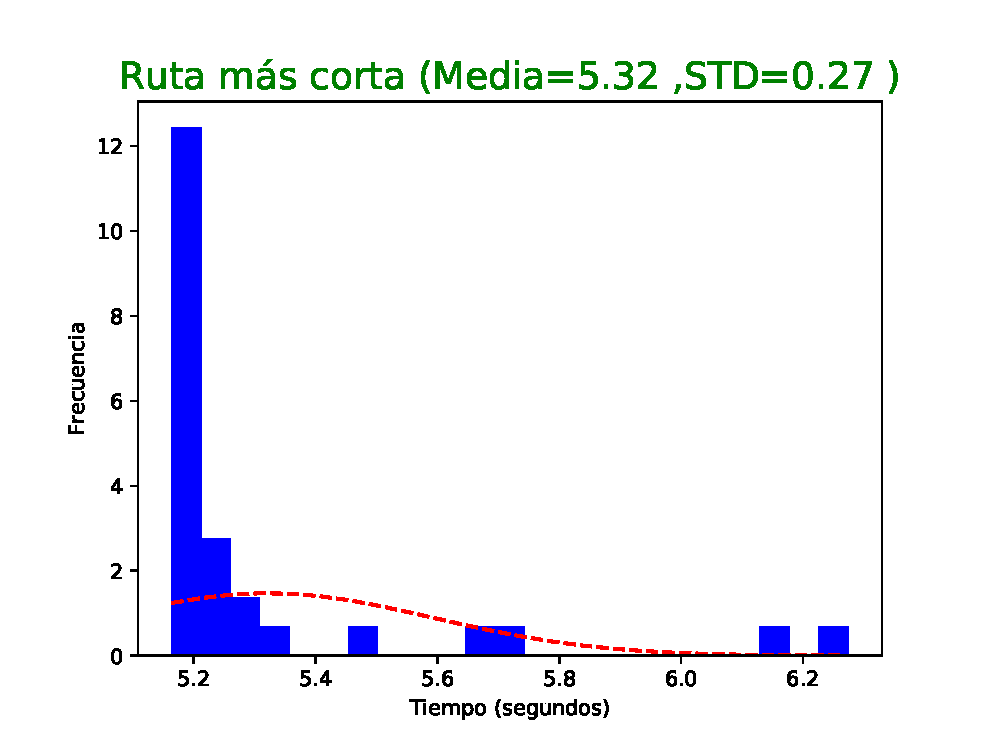
\includegraphics[width=\textwidth]{H1}
    \caption{Histograma para la ruta más corta.}
    \label{fig:H1}
\end{figure}
\begin{figure}[H]
    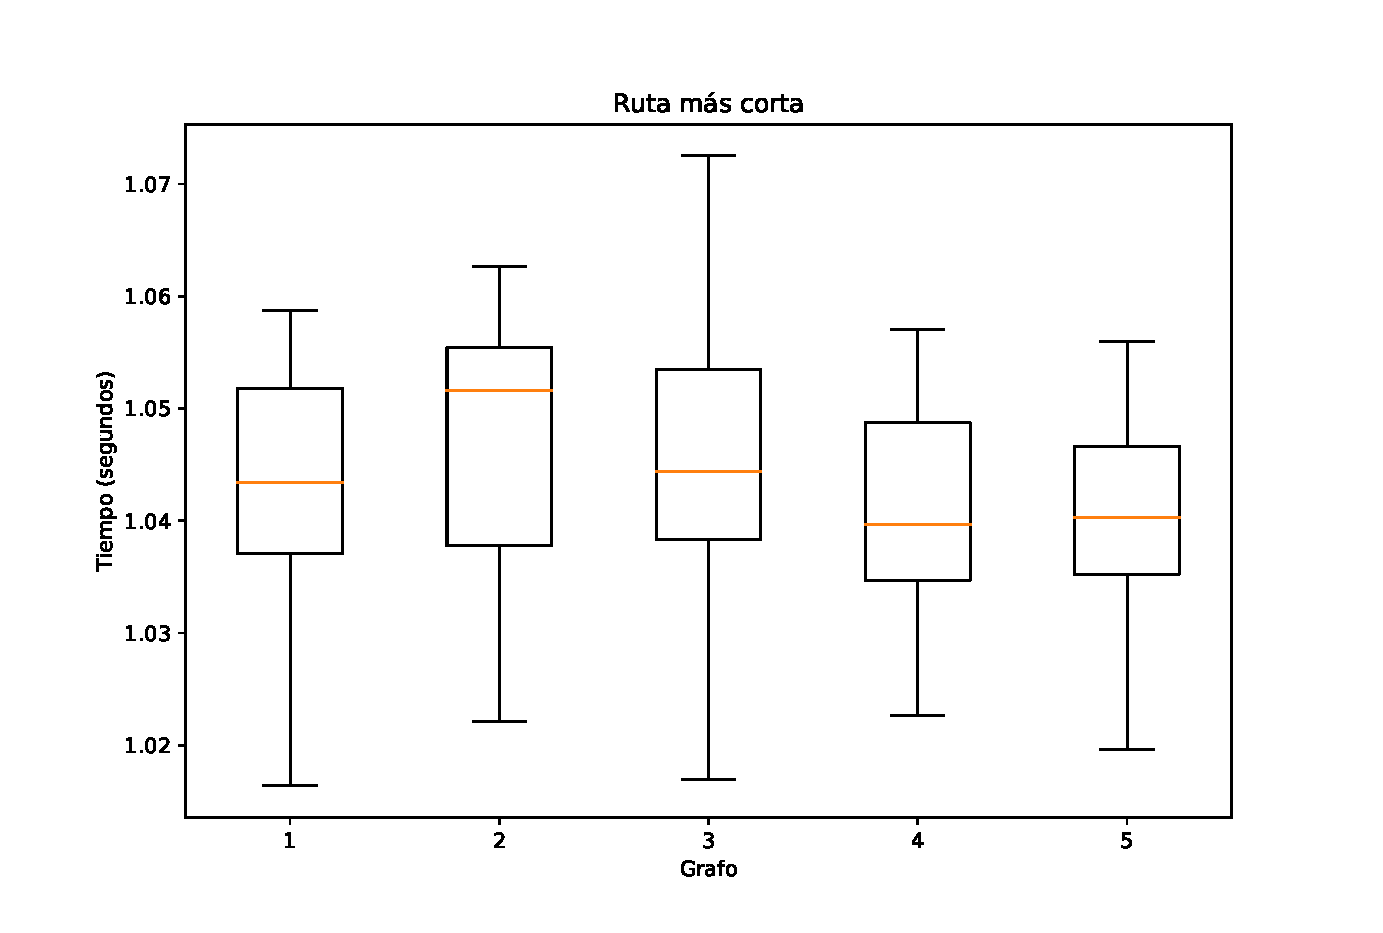
\includegraphics[width=\textwidth]{BP1}
    \caption{Diagrama caja y bigote para la ruta más corta.}
    \label{fig:BP1}
\end{figure}
\subsection{Árbol búsqueda a profundidad}
A continuación se muestra el histograma en la figura \ref{fig:H2} y el diagrama caja y bigote en la figura \ref{fig:BP2} con los resultados obtenidos:
\begin{figure}[H]
    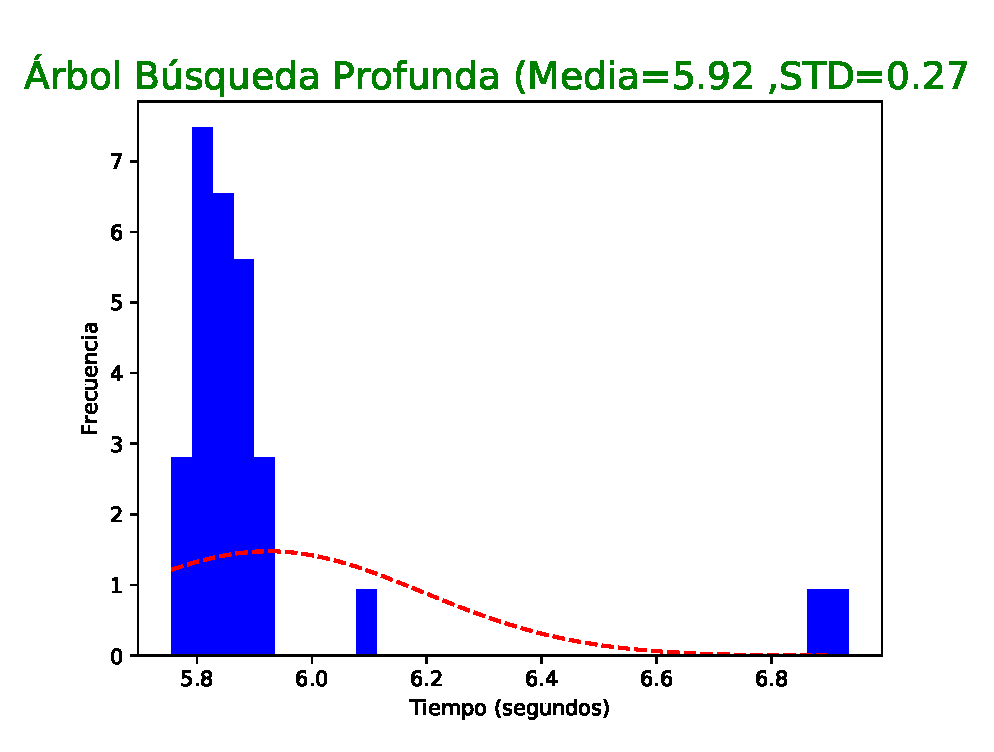
\includegraphics[width=\textwidth]{H2}
    \caption{Histograma para el árbol búsqueda a profundidad.}
    \label{fig:H2}
\end{figure}
\begin{figure}[H]
    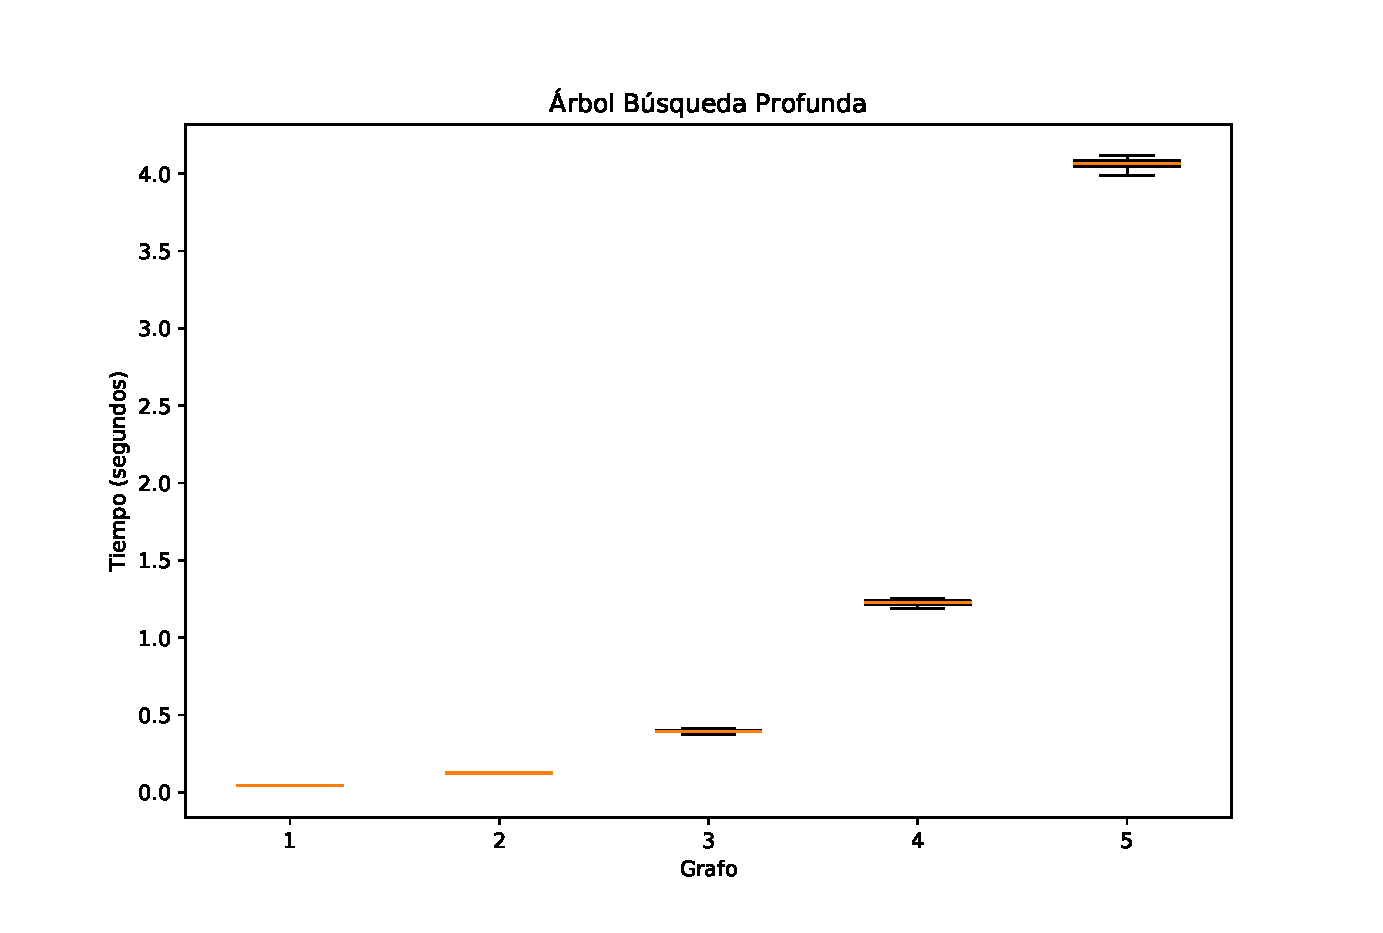
\includegraphics[width=\textwidth]{BP2}
    \caption{Diagrama caja y bigote para el árbol búsqueda a profundidad.}
    \label{fig:BP2}
\end{figure}
\subsection{Problema de la liga de amigos}
A continuación se muestra el histograma en la figura \ref{fig:H3} y el diagrama caja y bigote en la figura \ref{fig:BP3} con los resultados obtenidos:
\begin{figure}[H]
    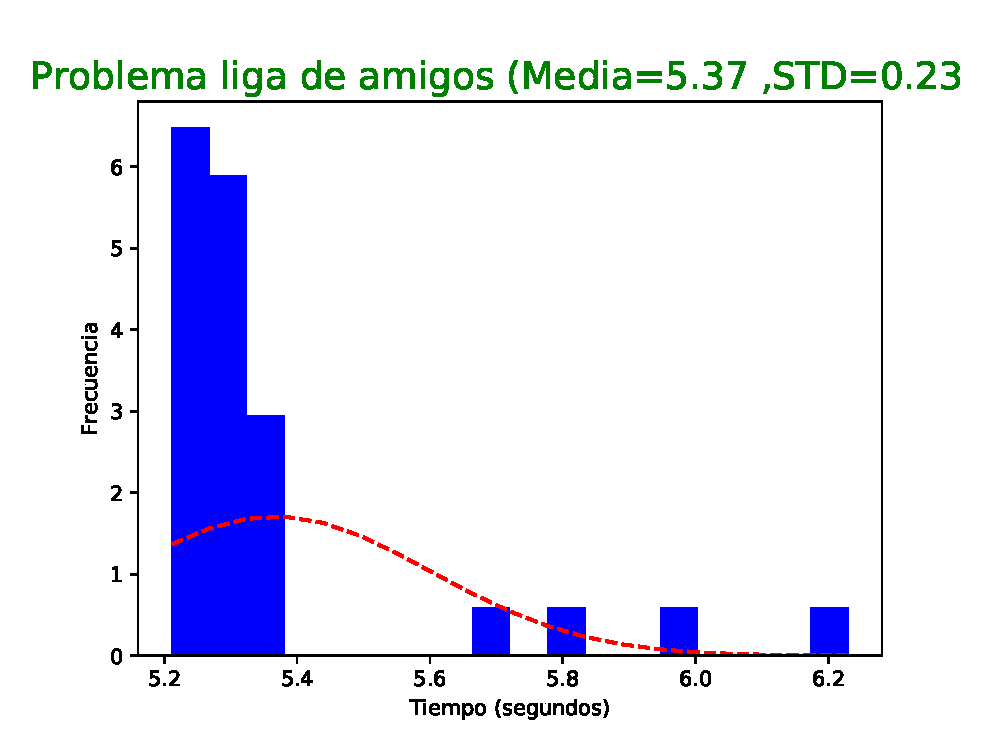
\includegraphics[width=\textwidth]{H3}
    \caption{Histograma para el problema de la liga de amigos.}
    \label{fig:H3}
\end{figure}
\begin{figure}[H]
    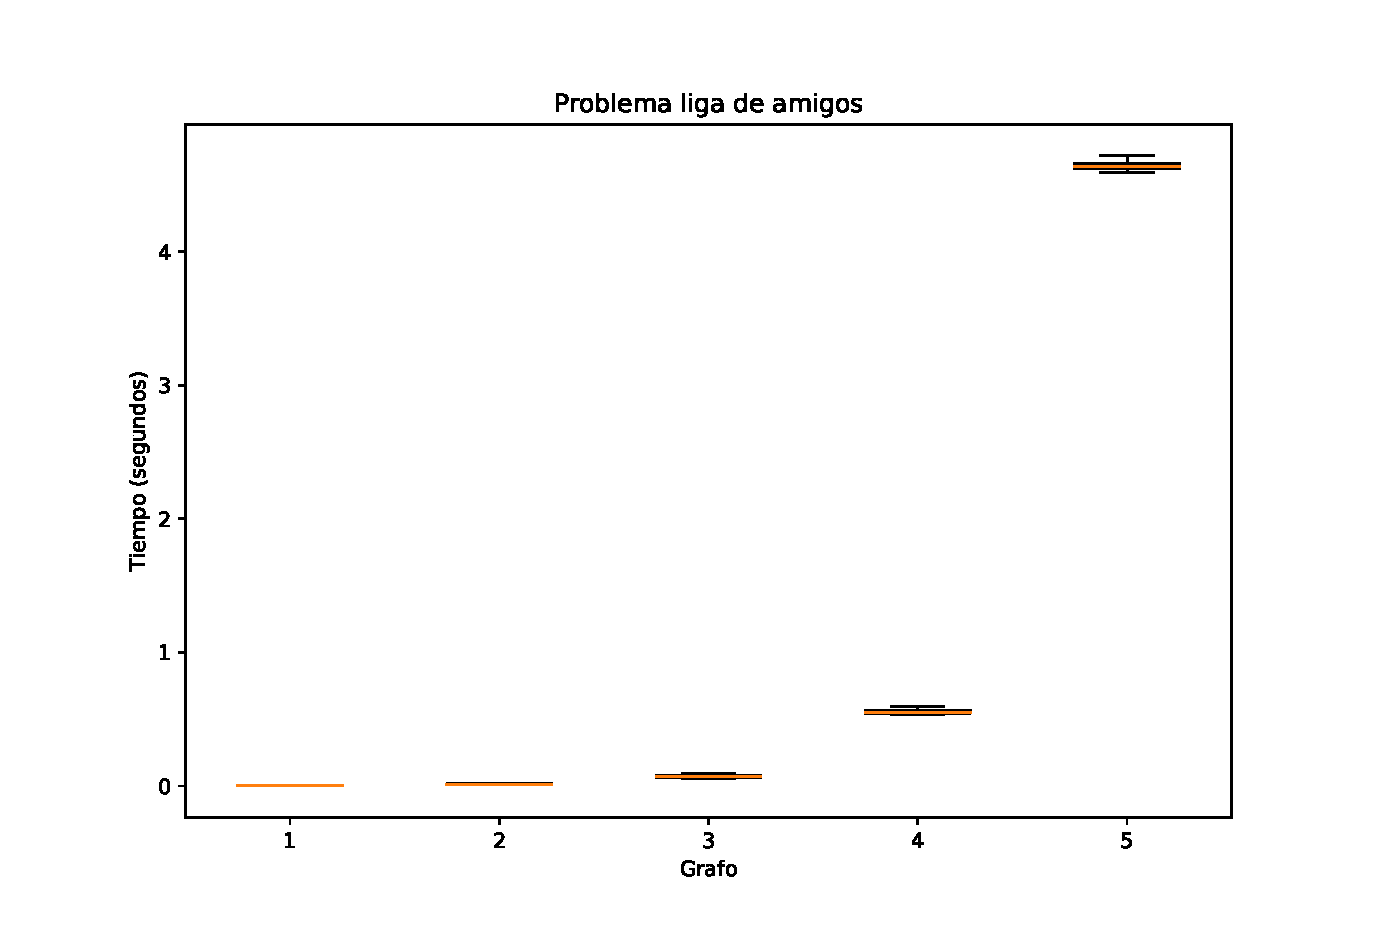
\includegraphics[width=\textwidth]{BP3}
    \caption{Diagrama caja y bigote para el problema de la liga de amigos.}
    \label{fig:BP3}
\end{figure}
\subsection{Árbol de mínimo grado}
A continuación se muestra el histograma en la figura \ref{fig:H4} y el diagrama caja y bigote en la figura \ref{fig:BP4} con los resultados obtenidos:
\begin{figure}[H]
    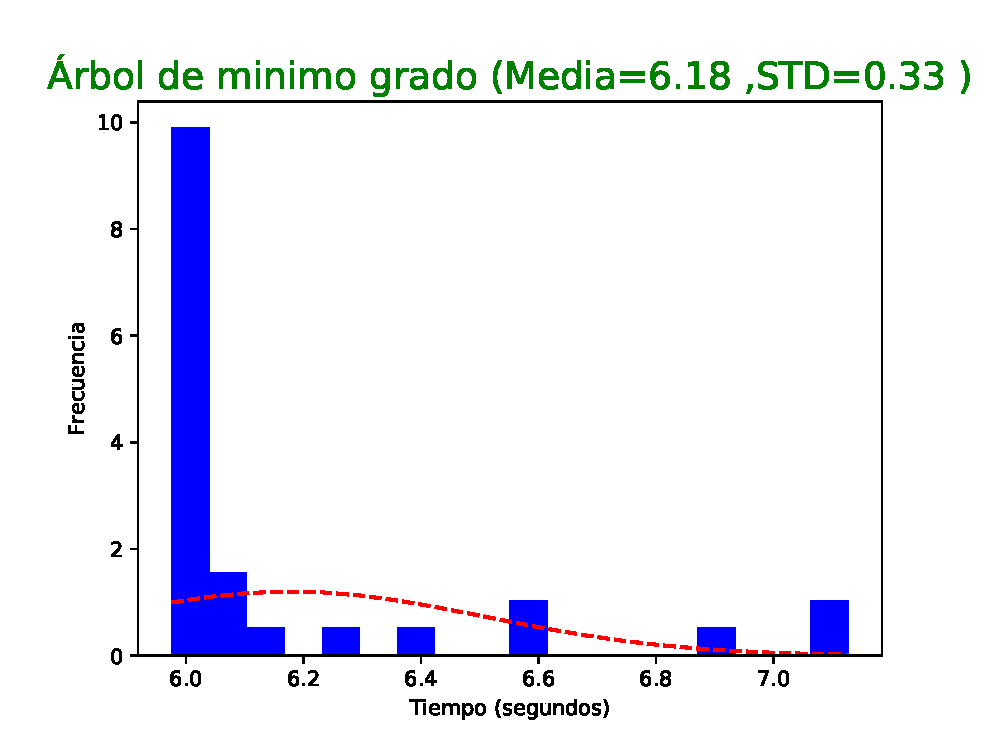
\includegraphics[width=\textwidth]{H4}
    \caption{Histograma para el árbol de mínimo grado.}
    \label{fig:H4}
\end{figure}
\begin{figure}[H]
    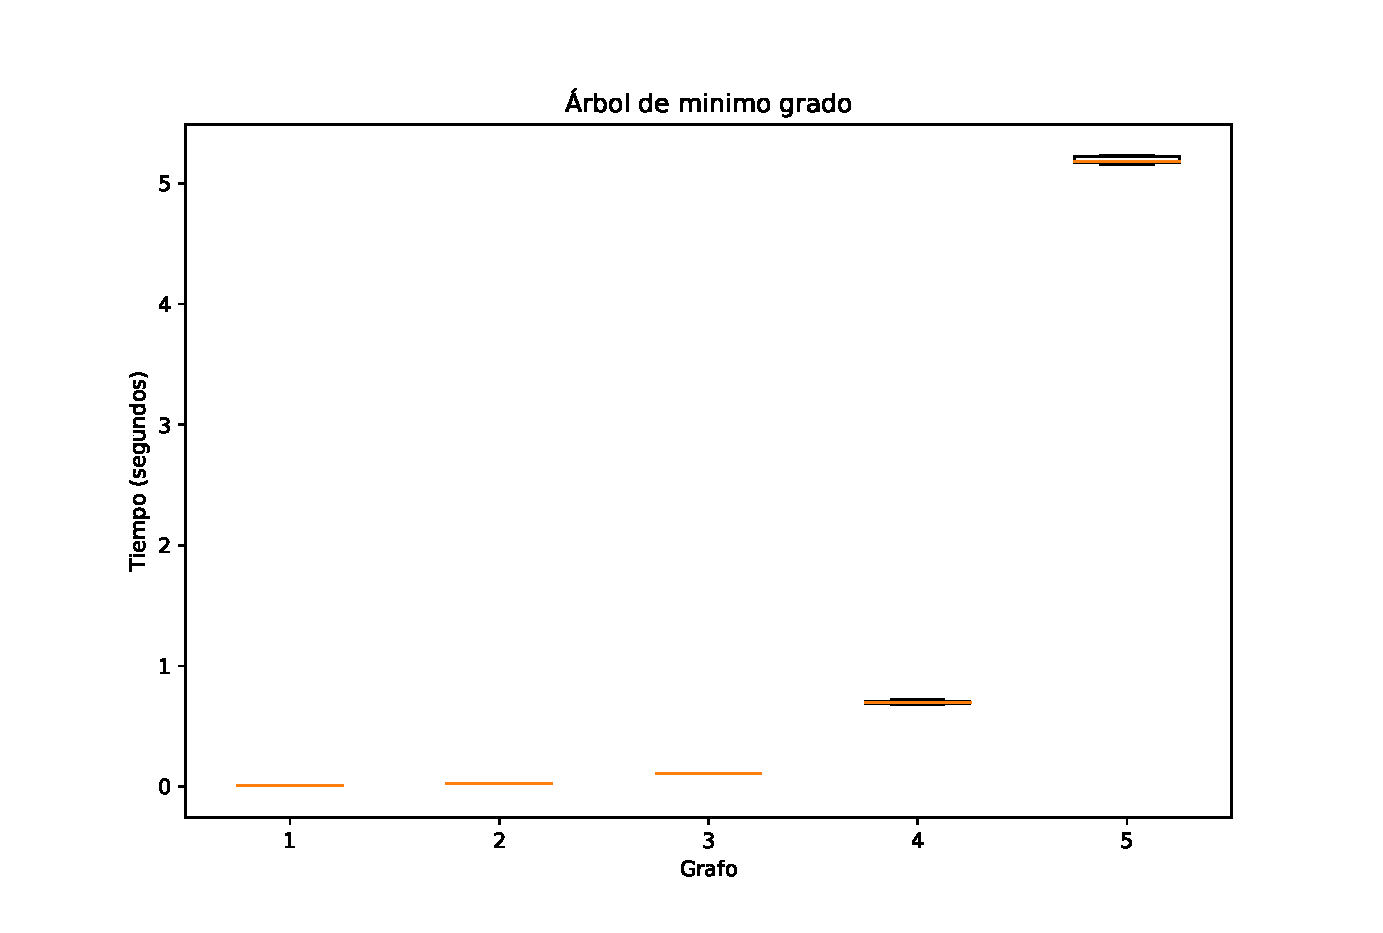
\includegraphics[width=\textwidth]{BP4}
    \caption{Diagrama caja y bigote para el árbol de mínima grado.}
    \label{fig:BP4}
\end{figure}
\subsection{Árbol de mínima expansión}
A continuación se muestra el histograma en la figura \ref{fig:H5} y el diagrama caja y bigote en la figura \ref{fig:BP5} con los resultados obtenidos:
\begin{figure}[H]
    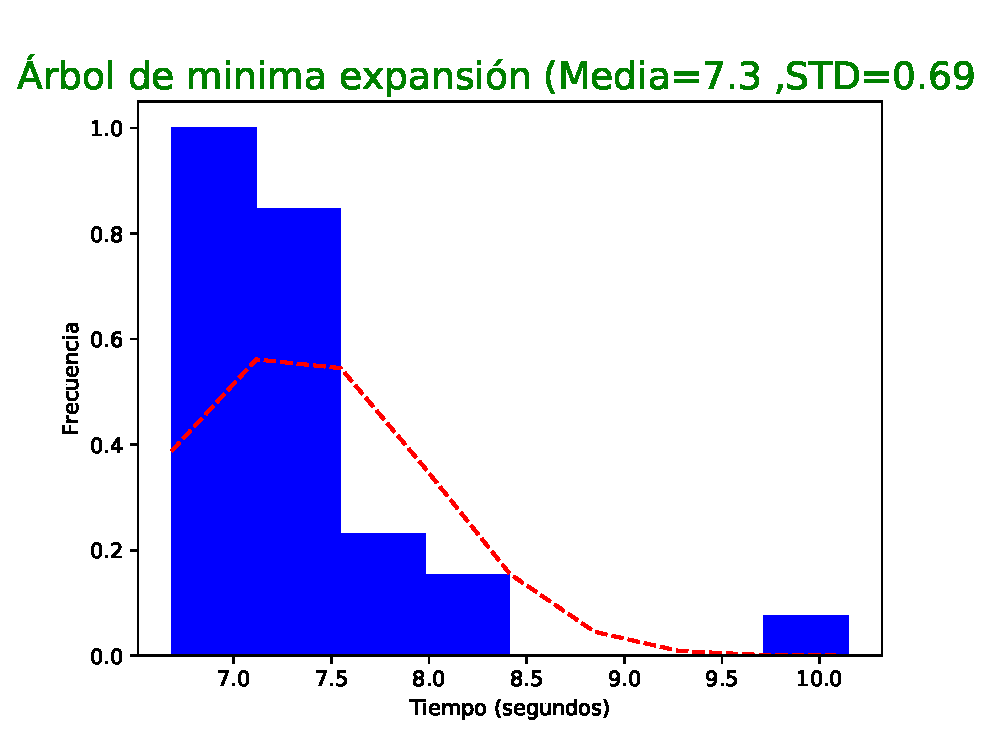
\includegraphics[width=\textwidth]{H5}
    \caption{Histograma para el árbol de mínima expansión.}
    \label{fig:H5}
\end{figure}
\begin{figure}[H]
    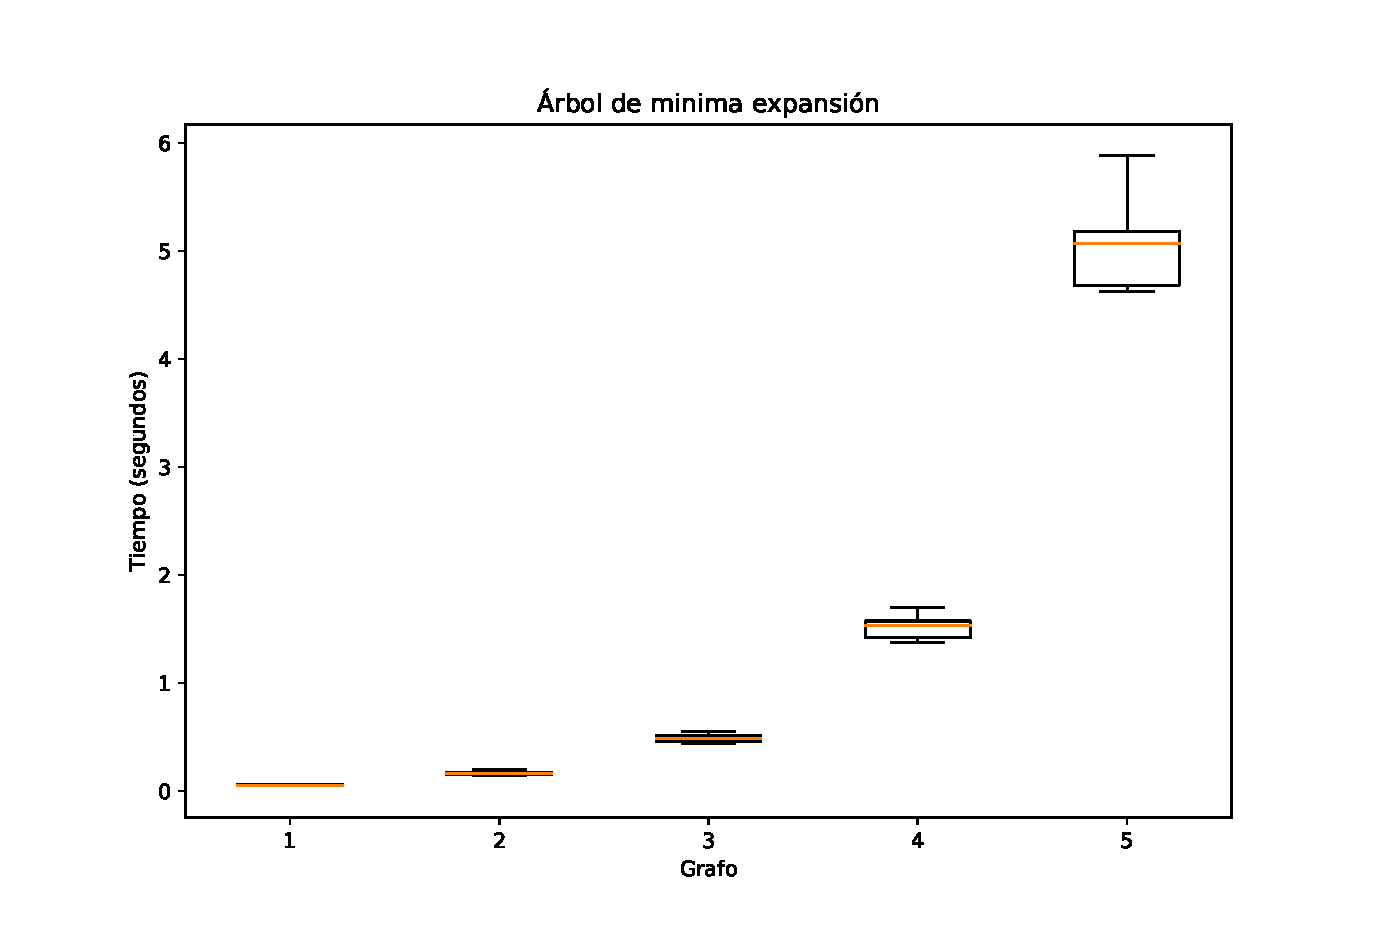
\includegraphics[width=\textwidth]{BP5}
    \caption{Diagrama caja y bigote para el árbol de mínima expansión.}
    \label{fig:BP5}
\end{figure}
\subsection{Comparación entre algoritmos}
La gráfica de dispersión siguiente compara los resultados obtenidos entre los 5 algoritmos, en base al tiempo de ejecución vs el número de nodos (figura \ref{fig:S1}) y el tiempo de ejecución vs el número de aristas (figura \ref{fig:S2}):

\begin{figure}[H]
    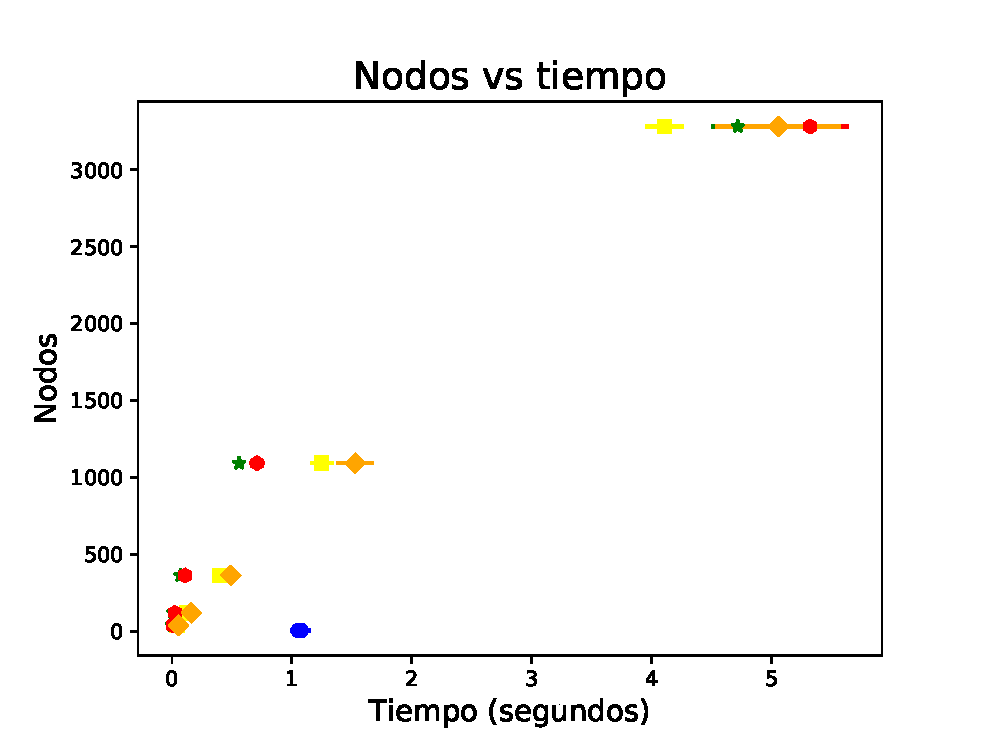
\includegraphics[width=\textwidth]{S1}
    \caption{Gráfica de dispersión: tiempo de ejecución vs número de nodos.}
    \label{fig:S1}
\end{figure}
\begin{figure}[H]
    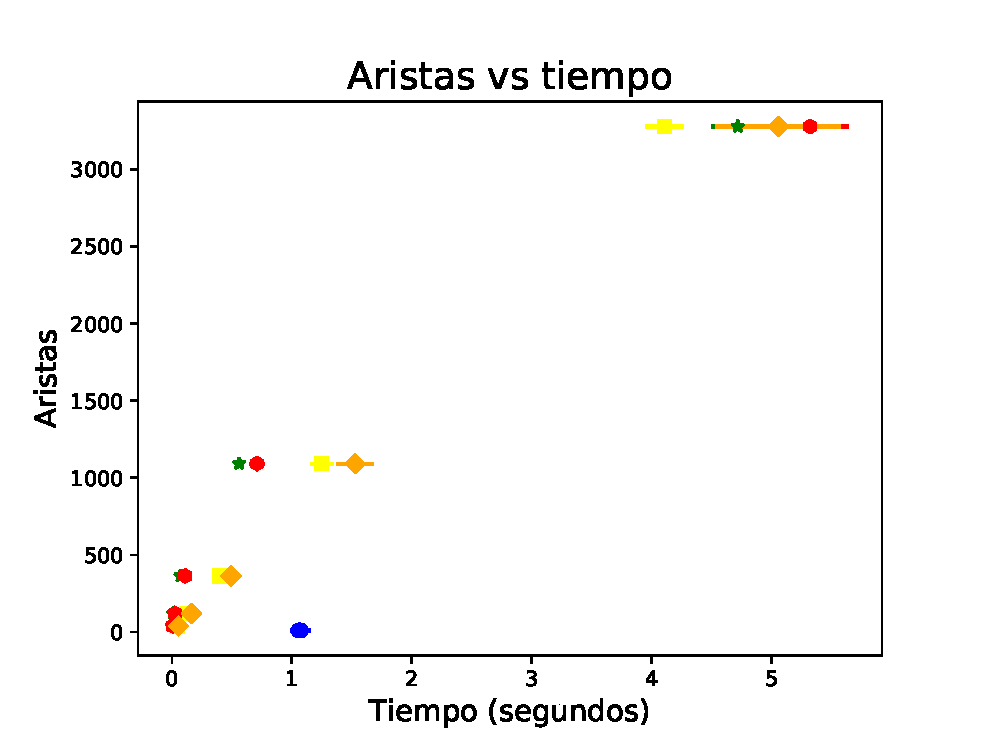
\includegraphics[width=\textwidth]{S2}
    \caption{Gráfica de dispersión: tiempo de ejecución vs número de aristas.}
    \label{fig:52}
\end{figure}
\section{Conclusiones}
Como conclusión de esta investigación, se tiene que el tiempo de ejecución de cualquiera de los 5 algoritmos estudiados es proporcional al número de nodos y de aristas que se tiene en el grafo, por lo que un grafo con un número mayor de nodos incrementa el tiempo de ejecución de los algoritmos.
\bibliographystyle{plain}
\bibliography{references}

\end{document}
